%!TEX root =  main.tex
\section{\dynastar: dynamic and quasi-optimum state partitioning}
%\section{\dynastar: dynamic partitioning for scalable state machine replication}
%\section{The centralized partitioning scheme}

%If the system can be modelled as a graph, as described in the previous session, we can take advantage of algorithms that perform graph partitioning to optimise the state partitioning of \ssmr\  while using concepts from \dssmr. The problem of graph partitioning is well stablished and despite being NP-Complete \ref{NPC_GraphPartition}, several approximation algorithms exist. First we define what graph partitioning is and how it can analysed to our needs, next we explore possibilities that are easily obtainable when applying the same graph's reasoning.

\subsection{Overview}
%\subsection{State partitioning as a graph problem}

We represent a service workload as a graph $G = (V, E)$, where vertices are state objects and an edges are operations.
There is an edge connecting two objects in the graph if a client can issue a command that accesses the objects. 




\subsection{The \dynastar protocol}

\begin{algorithm}[t!]
    \small

    \begin{distribalgo}[1]

        \vspace{1.5mm}

        \INDENT{\emph{Initialization:}}
            \STATE $round: 0$
            \STATE $new\_partitioning_{r}: \emptyset$
            \STATE $rcvd\_applies_{r} \leftarrow \emptyset$

        \ENDINDENT
        \vspace{1.5mm}
        \INDENT{Each oracle partition $o \in \oom$ does:}
            \vspace{1.5mm}
            \INDENT{\textbf{when} $receive(Partition)$}
                \STATE $round \leftarrow round + 1$
                \STATE $new\_partitioning_{round} \leftarrow$ partitioner($o.graph$)
                \STATE \rmcast$(\oom, Apply(round))$
            \ENDINDENT

            \vspace{1.5mm}

            \INDENT{\textbf{when} \rmdel$(Apply(round))$ from partition $o'$}
                \STATE $rcvd\_applies_{round} \leftarrow rcvd\_applies_{round} \cup o'$
                \IF{$rcvd\_applies_{round} \cap \oom = \emptyset$}
                    \STATE \amcast$(\oom, Apply(round))$
                \ENDIF
            \ENDINDENT

            \vspace{1.5mm}
            
             \INDENT{\textbf{when} \amdel$(Apply(round))$}
                \STATE $o.partitioning \leftarrow new\_partitioning_{round}$
            \ENDINDENT

        \ENDINDENT

    \vspace{1.7mm}

    \textbf{Algorithm variables:}

    \vspace{1.25mm}

    partitioner: An external partition algorithm

    \vspace{1.25mm}

    \oo: The set of oracle partitions

    \vspace{1mm}

    $o.graph$: The graph stored in the oracle

    \vspace{1mm}

    $o.partitioning$: The current graph partitioning

    \caption{Oracle's partitioning}
    \label{alg:oracle_partition}
\end{distribalgo}
\end{algorithm}


\begin{figure*}
\begin{minipage}[b]{1\linewidth} % A minipage that covers the whole width of the page
\centering
      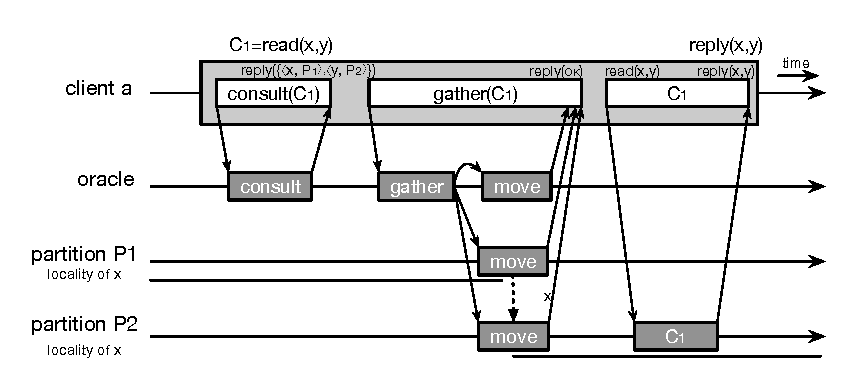
\includegraphics[width=1.0\linewidth]{figures/new-scheme}
\end{minipage}
\caption{How commands are treated in case of a repartitioning in the oracle.}
\label{fig:oracle_repartition}
\end{figure*}

%\begin{figure*}
%\begin{minipage}[b]{1\linewidth} % A minipage that covers the whole width of the page
%\centering
%      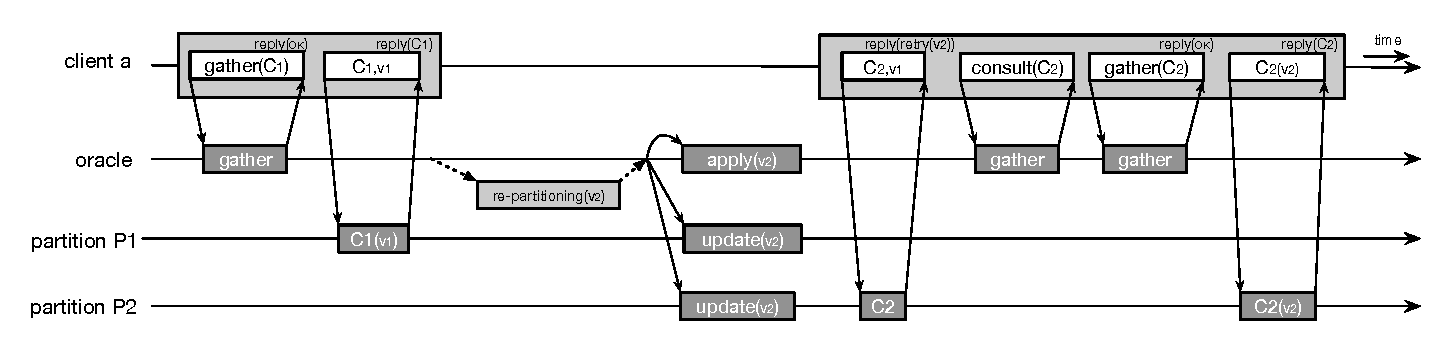
\includegraphics[width=1.0\linewidth]{figures/repartitioning}
%\end{minipage}
%\caption{How commands are treated in case of a repartitioning in the oracle.}
%\label{fig:oracle_repartition}
%\end{figure*}




\subsection{Correctness}
\label{sec:correctness}

In this section, we argue that \dssmr\ ensures termination and linearizability.
By ensuring termination, we mean that for every command $C$ issued by a correct client, a reply to $C$ different than $retry$ is eventually received by the client.
This assumes that at least one oracle process is correct and that every partition has at least one correct server.
Given these constraints, the only thing that could prevent a command from terminating would be an execution that forced the client proxy to keep retrying a command.
This problem is trivially solved by falling back to \ssmr\ after a predefined number of retries: at a certain point, the client proxy multicast the command to all server and oracle processes, which execute the command as in \ssmr{}, i.e., with coordination among all partitions and the oracle.

As for linearizability, we argue that, if every command in execution \ex\ of \dssmr\ is delivered by atomic multicast and is \emph{execution atomic} (as defined in~\cite{bezerra2014ssmr}), then \ex\ is linearizable.
We denote the order given by atomic multicast by relation $\prec$.
Given any two messages $m_1$ and $m_2$, ``$m_1 \prec m_2$'' means that there exists a process that delivers both messages and $m_1$ is delivered before $m_2$, or there is some message $m'$ such that $m_1 \prec m'$ and $m' \prec m_2$, which can be written as \mbox{$m_1 \prec m' \prec m_2$}.
%\fxnote[draft]{use the phrase \"there exists a process that\" }
Also, for the purposes of this proof, we consider the oracle to be a partition, as it also \amdel{}s and executes application commands.

Suppose, by means of contradiction, that there exist two commands $x$ and $y$, where $x$ finishes before $y$ starts, but $y \prec x$ in the execution.
There are two possibilities to be considered: (i) $x$ and $y$ are delivered by the same process $p$, or (ii) no process delivers both $x$ and $y$.

In case (i), at least one process $p$ delivers both $x$ and $y$.
As $x$ finishes before $y$ starts, then $p$ delivers $x$, then $y$. From the properties of atomic multicast, and since each partition is mapped to a multicast group, no process delivers $y$, then $x$.
Therefore, we reach a contradiction in this case.

In case (ii), if there were no other commands in \ex, then the execution of $x$ and $y$ could be done in any order, which would contradict the supposition that $y \prec x$.
Therefore, there are commands $z_1, ..., z_n$ with atomic order $y \prec z_1 \prec \cdots \prec z_n \prec x$, where some process $p_0$ (of partition $\ppm_0$) delivers $y$, then $z_1$; some process $p_1 \in \ppm_1$ delivers $z_1$, then $z_2$, and so on: process $p_i \in \ppm_i$ delivers $z_{i}$, then $z_{i+1}$, where $1 \leq i < n$.
Finally, process $p_n \in \ppm_n$ delivers $z_n$, then $x$.

Let $z_0 = y$ and let $atomic(i)$ be the following predicate:
``For every process $p_i \in \ppm_i$, $p_i$ finishes executing $z_i$ only after some $p_0 \in \ppm_0$ started executing $z_0$.''
We now claim that $atomic(i)$ is true for every $i$, where $0 \leq i \leq n$.
We prove our claim by induction.





